\begin{figure}[htp]
	\centering\capstart{}
	\subfloat[Initial Data]
	{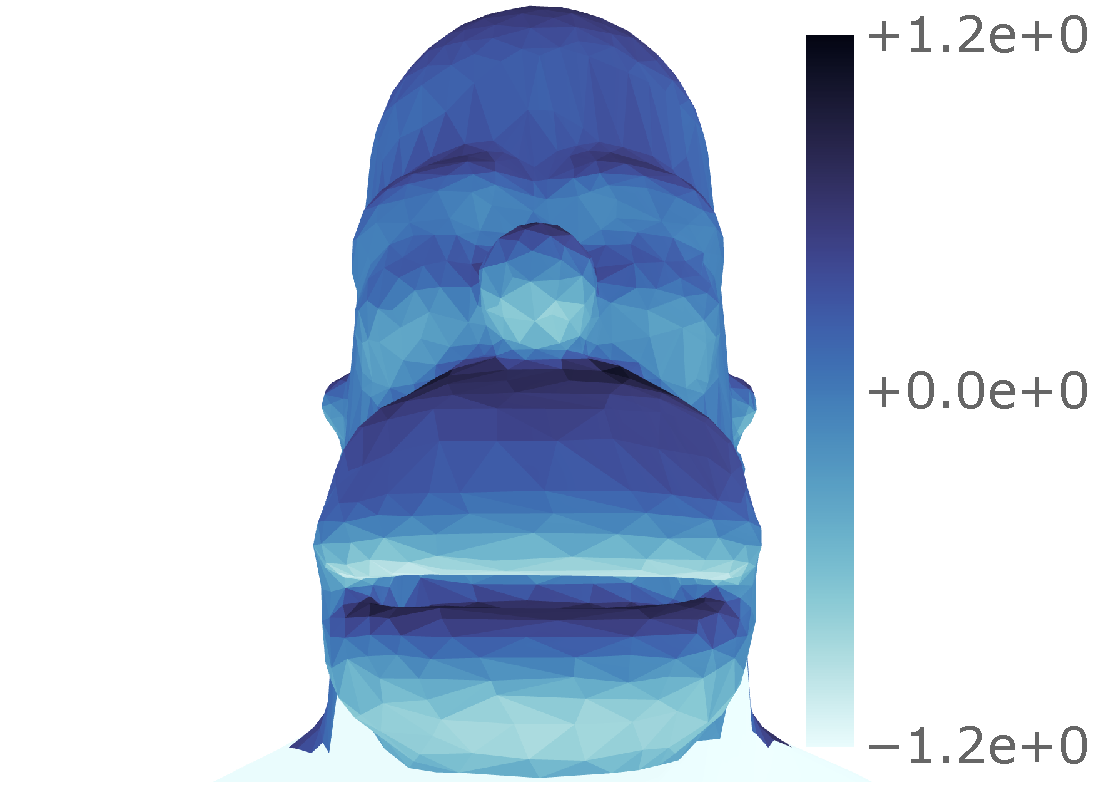
\includegraphics[trim={101 0 3 3},clip,width=.33\textwidth]{slepian_homer_field_zoom.pdf}}
	\hfill
	\subfloat[Noisy Data \newline
		\(\snr{z} = \SI{0.32}{\dB}\)]
	{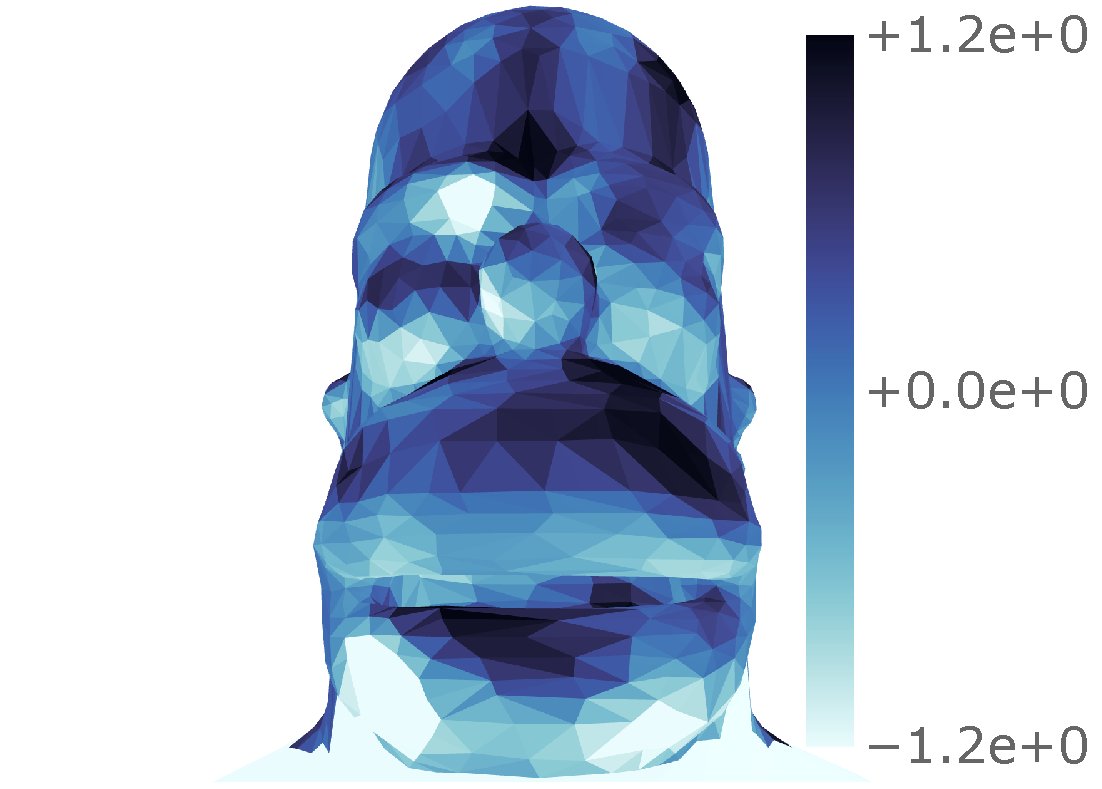
\includegraphics[trim={101 0 3 3},clip,width=.33\textwidth]{slepian_homer_field_-5noise_zoom.pdf}}
	\hfill
	\subfloat[Denoised \(N_{\sigma}=1\) \newline
		\(\snr{d} = \SI{2.29}{\dB}\)]
	{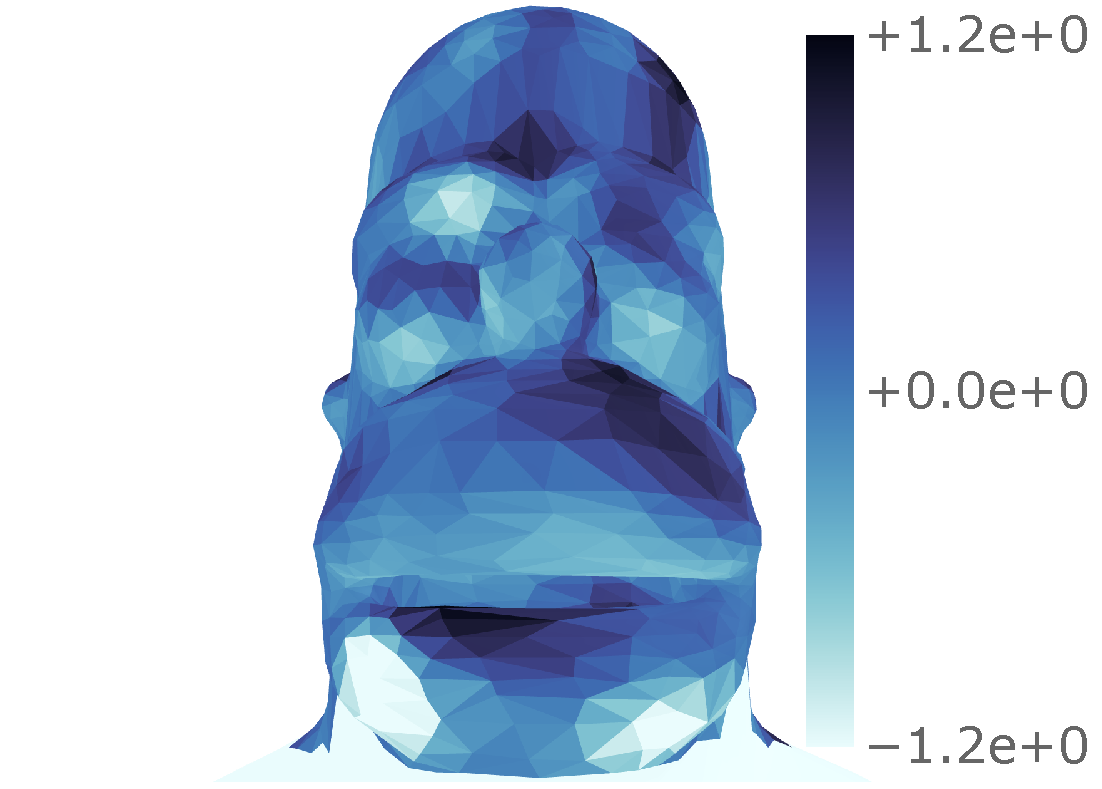
\includegraphics[trim={101 0 3 3},clip,width=.33\textwidth]{homer_-5snr_1n_denoised.pdf}}
	\caption[
		A denoising demonstration for a field on the Homer mesh
	]{
		Panel (a) shows the data in the region \(R\) constructed from the Slepian coefficients of the per vertex normals (\cf{} \cref{fig:chapter4_homer_data}) --- where the field value outside the region is set to negative infinity for illustrative purposes.
		Gaussian white noise is added to the signal in the Homer head region with a signal-to-noise ratio of \(\SI{0.32}{\dB}\), shown in panel (b).
		The scaling and wavelet coefficients of the noisy signal are calculated and are then hard-thresholded with \(N_{\sigma}=1\).
		The corresponding denoised plot is shown in panel (c), where the signal-to-noise ratio is boosted by \(\SI{1.97}{\dB}\) to \(\SI{2.29}{\dB}\).
		Whilst the signal values are defined on the vertices, they have been averaged onto the faces for the plot.
	}\label{fig:chapter4_denoising}
\end{figure}
